%
% Copyright (C) 2011 Agostino De Marco
%                    <agostino dot demarco at unina dot it>
%                    Roberto Giacomelli
%                    <giaconet dot mailbox at gmail dot com>
%
%    This work may be distributed and/or modified under the
%    conditions of the LaTeX Project Public License, either
%    version 1.3 of this license or any later version.
%    The latest version of this license is in
%    http://www.latex-project.org/lppl.txt and version 1.3
%    or later is part of all distributions of LaTeX version
%    2005/12/01 or later.
%
% This work has the LPPL maintenance status `maintained'.
% 
% The Current Maintainer of this work are Agostino De Marco
% and Roberto Giacomelli
%
\documentclass{standalone}
\usepackage{lmodern}
\usepackage{amsmath,fixmath}
\usepackage{relsize}
\usepackage{pgfplots}
\usepackage{siunitx}

\begin{document}

\pgfkeys{
   /pgf/number format/.cd,
      use comma
}
\pgfplotsset{
   every axis/.append style={
      font=\relsize{2},
      % very thick,% thick
      % tick style={very thick} % semithick
      line width=1.8pt,% thick
      tick style={line width=1.8pt} % semithick
      },
   every axis x label/.append style={
      font=\relsize{4},
      yshift=0pt,
      xshift=0em
   },
   every axis y label/.append style={
      font=\relsize{3},
      rotate=-90, % -90,
      xshift=-0.7em, % -0.2em,
      yshift=-1.4em, % 0.5em
   },
   major grid style={
      line width = 0.8pt,
      black,
      dash pattern=on 8pt off 4pt
   },
   every axis title/.append style={
      font=\relsize{3}
   }
}

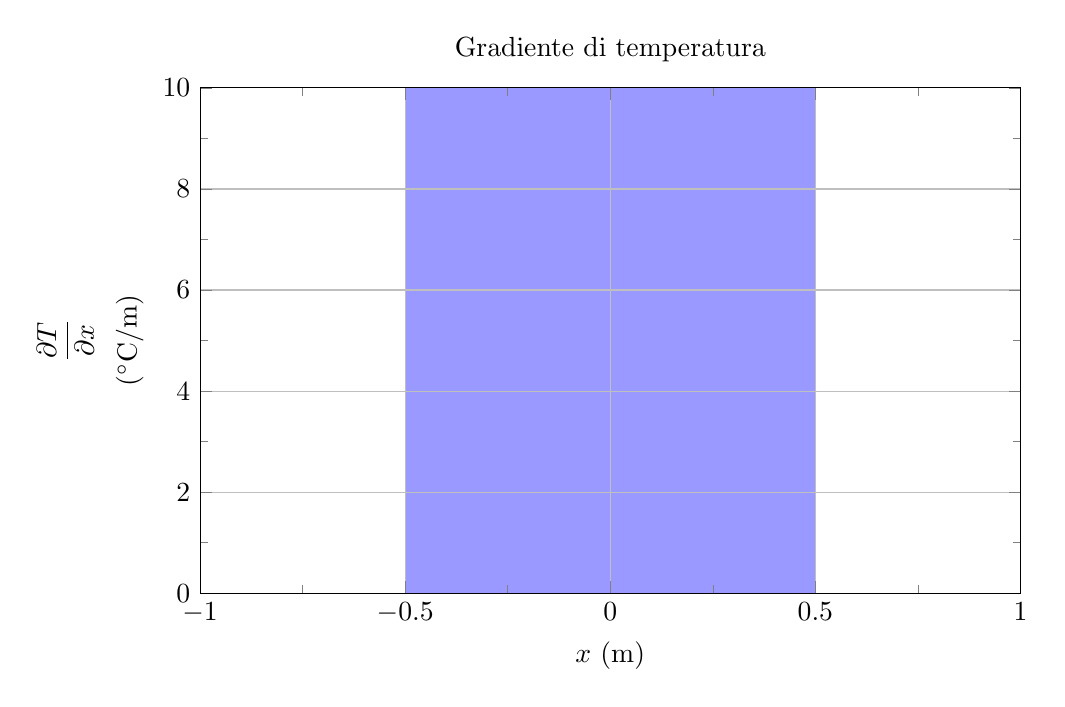
\begin{tikzpicture}
\begin{axis}[
   width=12cm,height=8cm,
   xmin=-1, xmax=1,
   ymin=0, ymax=10,
   xtick={-1,-0.5,...,1},
   ytick={0,2,...,10},
   minor x tick num = 1,
   minor y tick num = 1,
   grid=major,
   xlabel={$x$ (\si{\meter})},
   ylabel={
      \parbox{2cm}{%
               \centering
               $\dfrac{\partial T}{\partial x}$
               \\[0.7em]
               \centering
               (\si{\celsius/\meter})
      }
   },
   title=Gradiente di temperatura,
   axis on top=true
]

\fill[blue!40]
    (axis cs:-0.5,0) -- 
    (axis cs:0.5,0) -- 
    (axis cs:0.5,10) -- 
    (axis cs:-0.5,10) -- 
    cycle;

\end{axis}
\end{tikzpicture}
\end{document}